\section{Analog Front End} \label{sec:AnalogFrontEnd}

The analog front is a significant part of the impedance analyzer. The module is internally split into two major sections; a test signal generator and a sampling circuit. The module will generate test signals for the DUT with a digital-to-analog converter (DAC) and then acquire and sample the resulting DUT current and voltage waveforms with an analog-to-digital converter (ADC). A snippet of the analog front end can be seen on figure \refq{fig_6_1_AnalogFrontEnd}.

\begin{figure}[H]
    \centering
    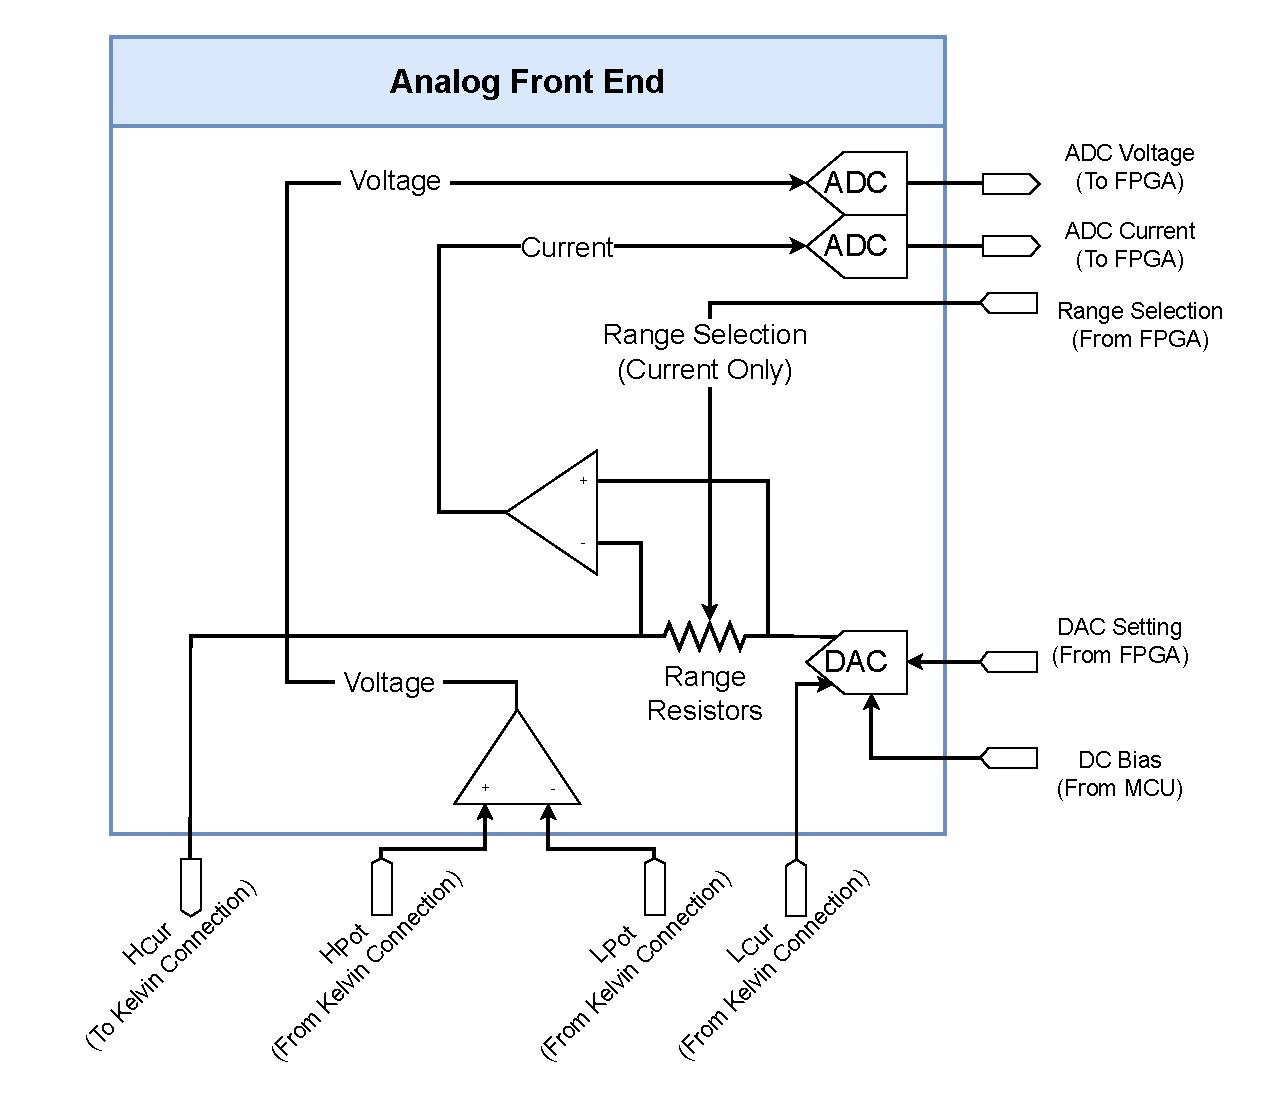
\includegraphics[clip, trim=18 0 18 0,width=0.70\textwidth]{Sections/6_SystemArchitecture/Figures/AnalogFrontEnd.pdf}
    \caption{The analog front end module. The DAC is generating the test signal for the DUT through the $H_{CUR}$, $L_{CUR}$ Kelvin Connections, while the two ADC's are sampling the DUT voltage through the $H_{pot}$ and $L_{pot}$ connections. The DUT current is sampled through a range resistor. All the control signal for the ADC and DAC come from the sample control module (marked as FPGA). The samples are stored in the sample control module. The  }
    \label{fig_6_1_AnalogFrontEnd}
\end{figure}

A DAC will generate the test signals for the DUT and the control signals for the DAC will come from the sample control module. The DAC will drive the DUT through a programmable gain amplifier, so it is possible to amplify the DAC output to ensure that the ADC always samples as large current and voltage signals as possible when the DUT's impedance is changing. This will allow the system to make use of the ADC's full dynamic range and increase the signal-to-noise ratio of the ADC. The DAC \textit{side} of the analog front end will have a system to DC bias the DUT as well, this means the DUT will see a sum of the test signal and DC bias voltage. The DC bias function is supplied by the Microprocessor module and will be described in section \refq{sec:MainProcessor}.

There are two ADC's in the module. ADC2 will acquire, and sample, the DUT current through a MUX'ed set of range resistors. A \textit{low} value of range resistor may be chosen if the DUT's impedance is low, and vice versa. The choice of range resistor will be decided by the sample control module, which will be described in section \refq{sec:Sample Control}. The sample control module will be controlling the choice of range resistor and the gain settings for the DAC's programmable amplifier. ADC1 will acquire, and sample, the voltage across the DUT. Both ADC1 and ADC2 will sample the current and voltage waveforms at the same time. The timing of this will be critical and is controlled by the sample control module.

The DAC and ADC's will have reconstruction and anti-aliasing filters. These are not shown on the block diagram but are assumed to be there.

The analog front end must interface with the Kelvin Connection, Sample Control and Main Processor modules, so their interfaces must be well defined. This will be shown in this section along with the modules specifications.

